\documentclass[12pt, a4paper, twoside, romanian]{teza-upb}
\setcounter{secnumdepth}{3}
\setcounter{tocdepth}{3}
% TikZ trebuie incarcat primul: pe TeX Live 2019, incarcarea bibliotecii
% arrows.meta dupa alte pachete (in special listings) provoaca erori
% "You can't use \unskip in vertical mode" la declararea sagetilor.
% xcolor se incarca cu optiunile sale INAINTEA lui tikz, altfel apare
% "Option clash for package xcolor" (tikz incarca xcolor fara optiuni).
\usepackage[svgnames,dvipsnames,x11names]{xcolor}
\usepackage{tikz}
\usetikzlibrary{positioning, shapes.geometric, arrows.meta}
\usepackage{babel}
\usepackage{graphicx}
\usepackage[
  bookmarks,
  bookmarksopen=true,
  unicode=true,
  pdfencoding=auto,
  pdftitle={Dizertatie},
  hidelinks,
  linktocpage]{hyperref}

\usepackage{url}

\usepackage[final]{pdfpages}


\usepackage{subcaption}

\usepackage[numbers,sort&compress]{natbib}
\usepackage{notoccite}

\usepackage{xurl}
\urlstyle{same}

\usepackage[normalem]{ulem}

\usepackage{amsmath,amsfonts,amssymb,amscd,amsthm}
\usepackage{mathtools}

\usepackage[tablename=Tabel]{caption}

\usepackage{soul}
\usepackage{booktabs}

\newcommand{\lt}{\ensuremath <}
\newcommand{\gt}{\ensuremath >}

\singlespacing

%%%%%%%%%%%%%%%%%%%%%%%%%%%%%%%%%%%%%%%%%%%%%%%%%%%%%%%%cod colorat
\usepackage{listings}
\usepackage{color}
 
\definecolor{codegreen}{rgb}{0,0.6,0}
\definecolor{codegray}{rgb}{0.5,0.5,0.5}
\definecolor{codepurple}{rgb}{0.58,0,0.82}
\definecolor{backcolour}{rgb}{0.95,0.95,0.92}

\lstdefinestyle{mystyle}{
	language=Matlab,
 %   backgroundcolor=\color{backcolour},   
    commentstyle=\color{codegreen},
    keywordstyle=\color{blue},
    numberstyle=\tiny\color{codegray},
    stringstyle=\color{codepurple},
	basicstyle=\ttfamily\scriptsize,
    breakatwhitespace=false,         
    breaklines=true,                 
    captionpos=b,                    
    keepspaces=true,                 
    numbers=left,                    
    numbersep=5pt,                  
    showspaces=false,                
    showstringspaces=false,
    showtabs=false,                  
    tabsize=2
}
 
\lstset{style=mystyle}

\usepackage{tabularx}

% -- Repoziționare număr de pagină în centru jos ------------------------
\makeatletter
\def\ps@topright{%
  \let\@mkboth\@gobbletwo    % nu punem nimic în header
  \def\@oddhead{}%
  \let\@evenhead\@oddhead
  % numărul în FOOTER, centrat
  \def\@oddfoot{\hfil\thepage\hfil}%
  \let\@evenfoot\@oddfoot
}
\makeatother

% -------- Nomenclature --------
\usepackage{nomencl}
\makenomenclature
\renewcommand{\nomname}{Lista acronimelor}

% To add nomenclature in the header
\renewcommand{\nompreamble}{\markboth{\nomname}{\nomname}}

% Add nomenclature to contents and print out nomenclature
\newcommand{\printnomencl}[1][]{
\ifthenelse{\equal {#1}{}}
{\printnomenclature}
{\printnomenclature[#1]}
%\addcontentsline{toc}{chapter}{\nomname}
}

% -------- Create the index --------
\makeindex


\usepackage{afterpage}
\newcommand\blankpage{
    \null
    \thispagestyle{empty}
    \newpage
}
%%%%%%%%%%%%%%%%%%%%%%%%%%%%%%%%%%%%%%%%%%%%%%%

\begin{document}

\author{Andreas BAȘCHIR}

\title{Sistem RAG pentru extragerea relațiilor între entități}
%va corespunde celui din Anexa 2, la care se poate adăuga un subtitlu


\facultatea{Facultatea de Electronică, Telecomunicații și Tehnologia Informației}
\tiplucrare{Proiect de diplomă}
%\tiplucrare{Lucrare de disertație}
\domeniu{Electronică și Telecomunicații}
\catedra{Electronică Aplicată și Ingineria Informației}
\campus{Leu} 
\program{Electronică Aplicată}
\titlulobtinut{Inginer}
%\titlulobtinut{Master}
\director{Ș.l. Dr. Ing. Liviu-Daniel ȘTEFAN \\
Drd. Fiz. Alexandru IONIȚĂ}

\submissionmonth{Iunie} 
\submissionyear{2026}

%\afterpage{\blankpage}
\beforepreface

\pagestyle{empty}
\listoffigures
\afterpage{\blankpage}
\listoftables
\afterpage{\blankpage}

\printnomenclature

\addcontentsline{toc}{chapter}{Lista acronimelor}
\nomenclature{CNN}{Convolutional Neural Network}
\nomenclature{DNN}{Deep Neural Network}

\afterpage{\blankpage}

\afterpreface 

% ======================================================
% CAPITOLE
% Fiecare capitol incepe pe pagina impara (conform regulamentului)
% ======================================================
\chapter*{Introducere}
\addcontentsline{toc}{chapter}{Introducere}

\section*{Scopul lucrării de diplomă} 

Sistemele RAG (Retrieval-Augmented-Generation) reprezintă o arhitectură de sistem de inteligență artificială care combină recuperarea informațiilor relevante din surse externe cu generarea de text de către modele de limbaj mari (LLMs - Large Language Models)

RAG a fost propus ca soluție pentru natura statică a informațiilor reținute de către modelele de limbaj mari, consecință a antrenării pe durate limitate, cu pauze între versiuni.  

\section*{Gradul de noutate}

Sistemele RAG au apărut oficial în 2020, prin lucrarea „Retrieval-Augmented Generation for Knowledge-Intensive NLP Tasks” publicată de Lewis et al. de la Facebook AI Research (astăzi Meta AI), în contextul exploziei modelelor transformer precum BERT și GPT, care generau răspunsuri creative, dar adesea inexacte sau „halucinate” din cauza limitărilor cunoștințelor lor statice.

De la începutul în 2020 cu RAG „naive”, sistemul a evoluat rapid: în 2023-2024 au apărut variante precum Advanced RAG și Modular RAG; în 2024, Microsoft a introdus GraphRAG pentru relații complexe via knowledge graphs, iar în 2025 s-au impus hibridări (vectori denși și rari, SQL-RAG pentru operații matematice) și Multi-RAG pentru scalabilitate în întreprinderile mari. Până în 2026, RAG este omniprezent în aplicații de business, chatbots și agenți AI, fiind o tehnologie utilizată în producție, trecută de ani de stadiul de prototip.

\section*{Obiectivele proiectului}

Obiectivul proiectului este de a introduce noțiuni despre contextul utilizării sistemelor RAG, cum se pot implementa, care sunt constrângerile dar și punctele forte ale acestora. Se vor prezenta și posibile direcții de viitor ale domeniului sistemelor RAG.

\section*{Contribuții și rezultate}

Se va prezenta o comparație utilizând metrici din mediul academic dintre un sistem RAG de tip "naive" și un sistem de tip "advanced", cu o interfață grafică de testare a LLM-urilor.

\section*{Conţinutul lucrării}

Lucrarea este structurată în două capitole principale:

\textbf{Capitolul 1 - Studiu de literatură} parcurge domeniul RAG din perspective teoretice și practice. Acesta cuprinde: (1) introducerea și contextul LLM-urilor în extragerea informației; (2) taxonomia sistemelor RAG clasificate după tipul recuperării, integrării și surselor de informație; (3) arhitectura generală a unui sistem RAG cu descrierea componentelor principale; (4) prezentarea metodelor și modelelor reprezentative din literatură (Self-RAG, CRAG, HyDE, GraphRAG); (5) definirea și analiza metricilor de evaluare pentru fiecare etapă a pipeline-ului de RAG (recuperare, generare, augmentare); (6) prezentarea seturilor de date utilizate în evaluarea RAG (T-REx, CRAG, WebNLG, HotpotQA); și (7) discutarea limitărilor și provocărilor actuale ale sistemelor RAG.

\textbf{Capitolul 2 - Rezultate experimentale} prezintă implementarea și comparația empirică a două tipuri de sisteme RAG: (1) Naive RAG - versiunea de bază cu recuperare pe bază de vectori denși și generare de către limbajul lingvistic mare; și (2) Advanced RAG - cu recuperare de tip hibrid, reordonare și rescriere a interogărilor LLM-ului. Pentru experimente a fost utilizat setul de date T-REx (relații entitate-entitate din Wikipedia aliniate cu Wikidata). Capitolul cuprinde atât analiza cantitativă (metrici RAGAS, Precision@K, Recall@K, MRR, F1) cât și analiza calitativă ale sistemelor RAG. Sistemele ilustrate anterior pot fi testate interactiv într-o interfață implementată în Streamlit.


\chapter{Studiu de literatură}

\section{Prezentarea domeniului lucrării de diplomă}

\subsection{Introducere}

Revoluția modelelor bazate pe arhitectura transformer, apărută în 2017~\cite{vaswani2017attention} și a limbajelor lingvistice mari (Large Language Models - LLMs) a dus la o schimbare paradigmatică a abordării problemelor de procesare de limbaj natural. Modele precum BERT și GPT-3 au demonstrat capacități remarcabile în înțelegerea și generarea de text coerent, ceea ce a dus la o adoptare rapidă a LLM-urilor global, cercetarea despre LLM-uri devenind un punct central de interes. În Figura 1.1 se pot observa modelele SOTA de-a lungul anilor 2018-2024. Totuși, LLM-urile de sine stătătoare au o limitare fundamentală, cunoștințele lor sunt fixe, limitate la momentul antrenării, neputând fi actualizate fără a fi reantrenate~\cite{gao2024retrievalaugmentedgenerationlargelanguage}.     

\begin{figure}
    \centering
    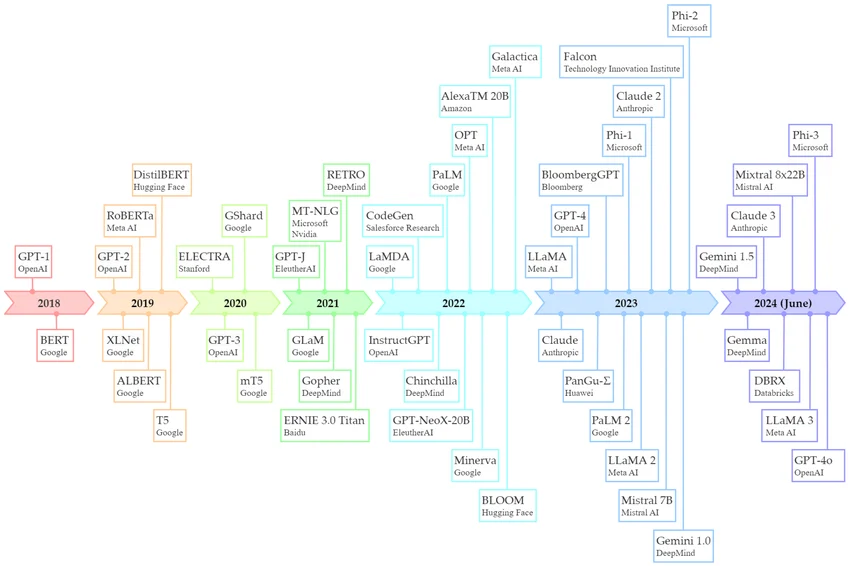
\includegraphics[width=1\linewidth]{Imagini/image.png}
    \caption{Evoluția modelelor lingvistice mari (LLMs) din 2018 până în 2024}
    \label{fig:placeholder}
\end{figure}

\subsection{Problema: Cunoștințe statice care duc la halucinații}

Fenomenul de „halucinație” reprezintă un răspuns aparent bine formulat, dar factual incorect, al unui LLM. Modelele generează text pe baza distribuției de probabilități a datelor cu care au fost antrenate, nu pe baza unor cunoștințe verificate. Pentru utilizatorul obișnuit, halucinațiile nu reprezintă un impediment major, însă există aplicații în care acestea sunt inacceptabile (medical, legal, financiar). 

În plus, informația încorporată în parametrii modelului este de natură „statică”, reflectă cunoștințele cunoscute la momentul antrenării. După antrenare, singura metodă de actualizare a informației este procesul costisitor de fine-tuning.

\subsection{Soluția: Retrieval-Augmented Generation}

Retrieval-Augmented Generation (RAG) este un tip de arhitectură de sistem de inteligență artificială care combină recuperarea informației relevante din surse externe cu capacitatea de generarea a LLM-urilor. În contextul unui sistem RAG, documentele relevante sunt recuperate dintr-o sursă externă de date, încorporate în contextul LLM-ului, iar în final, se generează un răspuns. Aceasta adresează ambele probleme simultan:

\begin{enumerate}
    \item Furnizează informația relevantă pentru un context factual corect, reducând astfel halucinațiile;
    \item Permite modificarea cunoștințelor și extensia contextului fără fine-tuning sau reantrenare.
\end{enumerate}

Termenul „RAG” a fost introdus în 2020 de către Patrick Lewis și colaboratorii săi de la Facebook AI Research (astăzi Meta AI) în lucrarea \textit{„Retrieval-Augmented Generation for Knowledge-Intensive NLP Tasks”}~\cite{lewis2020rag}.

\subsection{Formularea problemei: Extragerea relațiilor între entități}

Extragerea relațiilor între entități este o sarcină de bază în procesarea limbajului natural. Dat fiind un text, scopul este de a identifica entitățile menționate și relațiile dintre ele. De exemplu, din textul „Albert Einstein s-a născut în Ulm în 1879”, sistemul trebuie să extragă relațiile $(\text{Albert Einstein}, \text{născut în}, \text{Ulm})$ și $(\text{Albert Einstein}, \text{născut în an}, \text{1879})$.


Formal, fie $q$ o interogare și $\mathcal{D}=\{d_1,d_2,\dots,d_N\}$ o mulțime de documente. Un sistem RAG acționează în două etape. Prima etapă: un model de recuperare  $p_\eta(\cdot \mid q)$ alege o submulțime $\mathcal{Z} \subseteq \mathcal{D}$ de documente-candidat. A doua etapă: un model lingvistic mare generativ $p_\theta$ generează răspunsul $y$ condiționat de interogare dar și de documentele recuperate:
\begin{equation}
p(y \mid q) = \sum_{z \in \mathcal{Z}} p_\eta(z \mid q)\, p_\theta(y \mid q, z).
\label{eq:rag-marginal}
\end{equation}

RAG aduce o alternativă rețelelor neuronale de clasificare create pentru sarcini specifice. Sistemul recuperează pasaje relevante pentru fiecare pereche de entități, iar LLM-ul extrage relația pentru contextul recuperat, astfel generalizând pentru relații noi, fără reantrenare~\cite{gao2024retrievalaugmentedgenerationlargelanguage}.

\subsection{Relevanță și aplicații}

Sistemele RAG sunt relevante într-o gamă largă de domenii unde accesul dinamic la informații externe este esențial pentru generarea de răspunsuri de calitate~\cite{gao2024retrievalaugmentedgenerationlargelanguage}.
\begin{itemize}
    \item \textbf{Construirea grafurilor de cunoștințe}: Wikipedia, DBpedia, Freebase și alte baze de date semantice structurate sunt construite parțial prin extragerea automată a relațiilor
    \item \textbf{Asistenți inteligenți}: Chatbots și agenți de inteligență artificială care necesită cunoștințe actualizate constant
    \item \textbf{Domenii specializate}: Bioinformatică (extragerea relațiilor proteină-proteină), drept (identificarea precedenților), medicină (relații medicament-boală)
    \item \textbf{Indexare și căutare}: Motoarele de căutare moderne folosesc RAG pentru a livra răspunsuri directe
\end{itemize}

\section{Taxonomie}

\subsection{Motivația definirii unei taxonomii}

Domeniul RAG s-a dezvoltat rapid, producând numeroase variante și îmbunătățiri ale arhitecturii originale. Identificarea similarităților și diferențelor între abordări este dificilă fără o clasificare sistematică. Lucrările Gao et al. (2024) ~\cite{gao2024retrievalaugmentedgenerationlargelanguage} și Peng et al. (2025) ~\cite{peng2025graph} au fost folosite ca referință pentru această secțiune, care introduce o taxonomie bazată pe aspectele tehnologice cheie. Trebuie reținut că taxonomia este limitată la specificul acestei lucrări (RAG pentru extragerea relațiilor) și nu acoperă întreg domeniul.

\subsection{Criterii de clasificare}

\textbf{1. Tipul mecanismului de recuperare}

\begin{itemize}
    \item \textbf{Sparse retrieval}: Metode tradiționale de recuperare de IR (Information Retrieval) precum BM25, care se bazează pe potrivirea cuvintelor cheie. Rapid dar sensibil la variații lexicale și sinonime.
    \item \textbf{Dense retrieval}: Folosește reprezentări numerice a textului din documente (și interogarea către LLM) în spații vectoriale continue. Poate captura nuanțele semantice, dar costul computațional este mai ridicat.
    \item \textbf{Hybrid retrieval}: Combină sparse și dense prin fusion (ex. Reciprocal Rank Fusion), exploatând avantajele ambelor abordări. 
\end{itemize}

\textbf{2. Modul de integrare între recuperare și generare}

\begin{itemize}
    \item \textbf{Modular}: Componentele sunt decuplate. Recuperatorul și generatorul sunt independente și pot fi optimizate separat, oferind flexibilitate maximă.
    \item \textbf{End-to-end}: Recuperarea și generarea sunt cuplate, și sunt optimizate laolaltă, de regulă prin antrenare (gradient descent).
\end{itemize}

\textbf{3. Tipul sursei de cunoștințe}

\begin{itemize}
    \item \textbf{Nestructurată}: Documente text din diverse surse precum site-uri web (ex. articole Wikipedia), PDF-uri, documente Word. Pentru a putea fi procesate, necesită indexare și analiză semantică. 
    \item \textbf{Structurată}: Grafuri de cunoștințe cu entități și relații explicit modelate (DBpedia, Wikidata, Freebase), permitând navigare relațională.
    \item \textbf{Hibridă}: Combinație ale amândurora, exploatând avantaje complementare.
\end{itemize}

\textbf{4. Etapa augmentării}

\begin{itemize}
    \item \textbf{Pre-retrieval}: Optimizarea pre-recuperare prin extinderea și/sau reformularea interogării și descompunere semantică.
    \item \textbf{At-retrieval}: Optimizarea la momentul recuperării, prin selectarea parametrilor k, strategii adaptive de recuperare.
    \item \textbf{Post-retrieval}: Optimizare după recuperare, prin reranking, compactarea contextului și filtrare.
\end{itemize}

\subsection{Categorii principale}

\textbf{Naive RAG}

Paradigma originală din lucrarea Lewis et al. 2020~\cite{lewis2020rag}: indexare, urmată de recuperare de tip dense și generare. Recuperatorul și generatorul sunt elemente separate, și nu se folosesc optimizări. Este arhitectura de bază, folosită ca referință în majoritatea studiilor~\cite{lewis2020rag}, incluzând această teză. 

\textbf{Advanced RAG}

Adaugă optimizări pre- și post-recuperare, precum: rescriere a interogărilor, recuperare hibridă, și reranking cu model special antrenat. Dovedește îmbunătățiri semnificative, între 5 și 15\% pe benchmark-uri, cu costuri computaționale moderate. Lucrarea de față va implementa acest tip de arhitectură.

\textbf{Modular RAG}

Diferă de metodele Naive și Advanced în structură, fiecare element din arhitectura Modular RAG este un modul separat (ex. recuperare, memorare, rutare, predicție, căutare). Este cea mai adaptabilă/flexibilă arhitectură, însă introduce și cel mai înalt nivel de complexitate.

\textbf{Graph RAG}

Specifică pentru surse structurate de date: indexare pe grafuri de cunoștințe, recuperare utilizând relații semantice, generare pe bază de subgrafuri. Ideal pentru extragerea relațiilor din grafuri de cunoștințe dar necesită structurare prealabilă a datelor. Descris în detaliu de Peng et al. (2025)~\cite{peng2025graph}.

\section{Arhitectura generală a unui sistem de tip RAG}

Un sistem RAG funcționează în două faze: o fază offline de indexare și o fază online de inferență. Componentele principale sunt interogarea utilizatorului, baza de cunoștințe, mecanismul de recuperare și modelul generativ~\cite{gao2024retrievalaugmentedgenerationlargelanguage}.

\subsection{Componentele sistemului}

\textbf{Interogarea} reprezintă nevoia de informație a utilizatorului. În formele de bază, textul interogării este transmis direct mecanismului de recuperare. Sistemele avansate aplică mai întâi transformări ale interogării: reformulare semantică, extindere cu termeni sinonimi sau descompunere în sub-interogări, pentru a crește acoperirea și a reduce sensibilitatea față de formulări ambigue~\cite{gao2024retrievalaugmentedgenerationlargelanguage}.

\textbf{Baza de cunoștințe} este sursa externă din care se extrage informația. Documentele trec printr-o etapă de indexare offline: sunt împărțite în fragmente (eng. \textit{chunks}), codificate cu un model de reprezentare vectorială bazat pe arhitectura transformer~\cite{vaswani2017attention} și stocate într-o bază de date vectorială~\cite{karpukhin2020dpr}. Strategia de fragmentare influențează direct calitatea recuperării: fragmentele prea scurte pierd contextul necesar pentru identificarea relațiilor între entități, iar cele prea lungi diluează semnalul relevant.

\textbf{Mecanismul de recuperare} punctează fragmentele din baza vectorială în raport cu interogarea și returnează primele $k$ rezultate. Sistemele dense calculează similaritatea cosinus între vectorul interogării și vectorii fragmentelor~\cite{karpukhin2020dpr}. Sistemele sparse aplică potrivire ponderată de termeni, BM25 reprezentând standardul din domeniu~\cite{robertson2009bm25}. Sistemele hibride combină scorurile dense și sparse prin Reciprocal Rank Fusion (RRF)~\cite{cormack2009rrf}. Opțional, un model de reranking de tip cross-encoder poate rafina ordinea inițială a fragmentelor recuperate.

\textbf{Modelul generativ} primește contextul augmentat, format din interogarea originală și fragmentele recuperate, și produce răspunsul final~\cite{lewis2020rag}. Arhitecturile orientate spre fidelitate constrâng explicit modelul să fundamenteze răspunsurile pe dovezile recuperate, reducând astfel rata de halucinații~\cite{asai2023self}.

\subsection{Fluxul de date}

Figura~\ref{fig:rag-arch} ilustrează cele două trasee ale fluxului de date. Offline, documentele sunt procesate o singură dată: fragmentate, codificate și stocate în baza vectorială. Online, fiecare interogare parcurge procesarea interogării, recuperarea fragmentelor, augmentarea contextului și generarea răspunsului.

\begin{figure}[htbp]
    \centering
    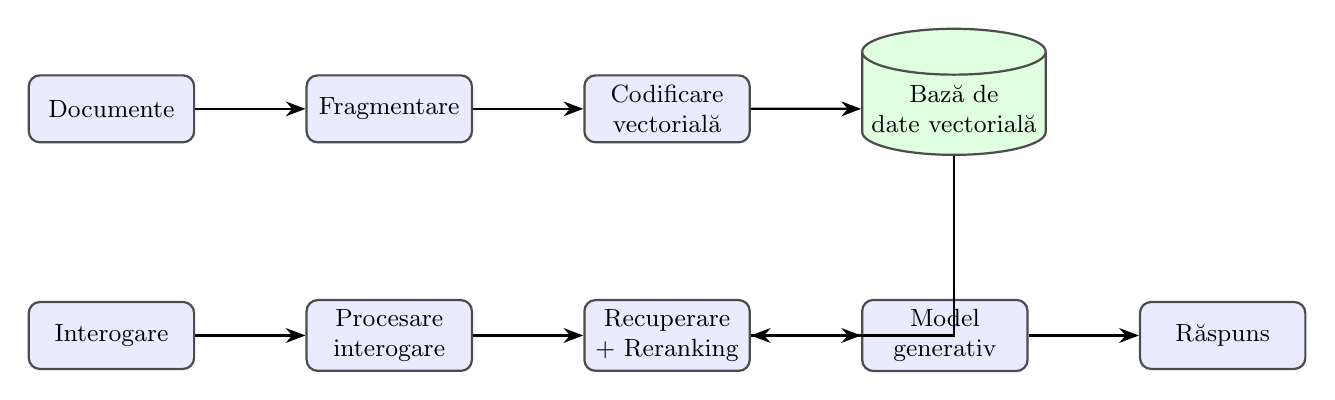
\begin{tikzpicture}[
        node distance=1.0cm and 1.4cm,
        proc/.style={rectangle, rounded corners, draw=black!70, fill=blue!8, thick, align=center, minimum width=2.1cm, minimum height=0.85cm, font=\small},
        store/.style={cylinder, shape border rotate=90, aspect=0.25, draw=black!70, fill=green!12, thick, align=center, minimum width=2.1cm, font=\small},
        arr/.style={-{Stealth[length=2.5mm]}, thick}
    ]
    \node[proc] (docs) {Documente};
    \node[proc, right=of docs] (chunk) {Fragmentare};
    \node[proc, right=of chunk] (emb) {Codificare\\vectorială};
    \node[store, right=of emb] (vdb) {Bază de\\date vectorială};
    \draw[arr] (docs) -- (chunk);
    \draw[arr] (chunk) -- (emb);
    \draw[arr] (emb) -- (vdb);
    \node[proc, below=2.0cm of docs] (query) {Interogare};
    \node[proc, right=of query] (qproc) {Procesare\\interogare};
    \node[proc, right=of qproc] (retr) {Recuperare\\+ Reranking};
    \node[proc, right=of retr] (gen) {Model\\generativ};
    \node[proc, right=of gen] (out) {Răspuns};
    \draw[arr] (query) -- (qproc);
    \draw[arr] (qproc) -- (retr);
    \draw[arr] (retr) -- (gen);
    \draw[arr] (gen) -- (out);
    \draw[arr] (vdb) |- (retr);
    \end{tikzpicture}
    \caption{Arhitectura generală a unui sistem RAG: indexare offline (sus) și inferență online (jos)~\cite{gao2024retrievalaugmentedgenerationlargelanguage, karpukhin2020dpr}.}
    \label{fig:rag-arch}
\end{figure}

\section{Metode și modele RAG}

\subsection{Naive RAG}

Formularea originală a RAG, propusă de Lewis et al. (2020)~\cite{lewis2020rag}, combină un recuperator bazat pe Dense Passage Retrieval (DPR) cu un model generativ de tip sequence-to-sequence, optimizate parțial în comun. Fluxul de lucru este liniar: indexare, recuperare densă, generare. Această variantă servește ca referință în majoritatea studiilor din literatura de specialitate~\cite{gao2024retrievalaugmentedgenerationlargelanguage}.

Limitările Naive RAG sunt bine documentate: sistemul nu gestionează variațiile lexicale (sinonime, parafrazări), nu evaluează calitatea documentelor recuperate și nu filtrează fragmentele irelevante înainte de generare~\cite{gao2024retrievalaugmentedgenerationlargelanguage}. Cu toate acestea, simplitatea sa face din Naive RAG un punct de plecare util pentru orice evaluare comparativă, inclusiv în cadrul acestei teze.

\subsection{Advanced RAG}

Advanced RAG adaugă optimizări pre-recuperare și post-recuperare față de varianta de bază~\cite{gao2024retrievalaugmentedgenerationlargelanguage}. Pre-recuperare: fragmentare semantică, îmbogățirea fragmentelor cu metadate, generare de interogări multiple. Post-recuperare: reranking cu model cross-encoder, compactarea contextului pentru a reduce zgomotul din prompt. Scorurile dense și sparse sunt combinate prin RRF~\cite{cormack2009rrf}. Studiile raportează îmbunătățiri de 5--15\% față de Naive RAG pe benchmark-uri standard.

Pentru extragerea relațiilor, optimizările post-recuperare sunt relevante în mod direct: identificarea corectă a unei relații necesită fragmente care conțin simultan ambele mențiuni de entitate și indiciile lexicali ai relației. Reranking-ul crește șansa ca aceste fragmente să ajungă în contextul modelului generativ. Aceasta este arhitectura pe care lucrarea de față o implementează și evaluează în partea experimentală.

\subsection{Hypothetical Document Embeddings (HyDE)}

HyDE~\cite{gao2023hyde} folosește un model de limbaj pentru a genera un pseudo-document care ar conține răspunsul la interogare. Acest pseudo-document este codificat și se caută documente reale similare prin recuperare densă. Encoderele contrastive eliminată erorile factuale din pseudo-document, păstrând tiparele de relevanță semantică~\cite{gao2023hyde}.

Avantajul principal al HyDE este că îmbunătățește recuperarea fără a necesita date de antrenare etichetate pentru interogări. Dezavantajul este dependența de calitatea generării inițiale: un pseudo-document slab generat poate conduce recuperarea în direcția greșită.

\subsection{REALM, Fusion-in-Decoder și RETRO}

REALM~\cite{guu2020realm} integrează recuperarea chiar în etapa de pre-antrenare, tratând recuperatorul ca o variabilă latentă optimizată împreună cu modelul de limbaj. Abordarea arată că un recuperator co-antrenat cu generatorul înțelege mai bine ce tipuri de documente sunt utile pentru diferite sarcini.

Fusion-in-Decoder (FiD)~\cite{izacard2021fid} codifică fiecare pasaj recuperat independent prin encoder, dar realizează fuziunea la nivelul decoderului. Astfel, modelul poate agrega dovezi din surse multiple fără a sufoca encoderele cu un context prea lung. RETRO~\cite{borgeaud2022retro} extinde această idee la scara corpusurilor de zeci de trilioane de tokenuri, fără a crește proporțional numărul de parametri ai modelului, obținând eficiență parametrică pe seama unei infrastructuri mai complexe.

\subsection{RAPTOR}

RAPTOR~\cite{sarthi2024raptor} construiește un arbore de rezumate de jos în sus: fragmentele de text sunt grupate în clustere, rezumate, iar procesul se repetă recursiv, generând niveluri de abstractizare din ce în ce mai înalte. La inferență, recuperarea operează pe acest arbore și poate agrega informații de la mai multe niveluri de abstractizare simultan.

Metoda obține rezultate bune pe sarcini care necesită raționament distribuit pe mai multe documente~\cite{sarthi2024raptor}. Avantajul față de recuperarea standard este că furnizează modelului generativ atât detalii de granularitate fină, cât și context global. Dezavantajul constă în costul de construire și actualizare a arborelui.

\subsection{Corrective RAG (CRAG)}

CRAG~\cite{yan2024crag} adaugă un evaluator al calității documentelor recuperate. Când relevanța fragmentelor este insuficientă, sistemul declanșează acțiuni corective: recuperare suplimentară sau căutare pe web, urmată de rafinarea cunoștințelor prin descompunere și recompunere a informației. Dacă documentele recuperate sunt de bună calitate, fluxul rămâne cel standard.

Mecanismul de auto-corecție face sistemul mai robust față de recuperările greșite și reduce riscul extragerii unei relații dintr-un context irelevant. CRAG este una dintre primele abordări care tratează explicit eșecul recuperării ca un caz de gestionat, nu ca o excepție rară.

\subsection{Self-RAG}

Self-RAG~\cite{asai2023self} antrenează un singur model să decidă adaptiv când să recupereze, când să genereze și când să critice propriile răspunsuri, folosind tokenuri speciale de reflecție introduse în vocabularul modelului. Modelul evaluează relevanța fragmentului recuperat și gradul de fundamentare factuală a răspunsului generat înainte de a-l returna utilizatorului.

Față de CRAG, care utilizează un evaluator extern, Self-RAG internalizează întregul proces de evaluare și corecție. Fidelitatea și controlabilitatea cresc~\cite{asai2023self}. Pentru extragerea relațiilor, posibilitatea de a verifica dacă tipul de relație prezis este susținut de dovezile recuperate este utilă în mod direct, deoarece reduce numărul de relații extrase din fragmente slab relevante.

\subsection{Adaptive-RAG și FLARE}

Adaptive-RAG~\cite{jeong2024adaptiverag} alege dinamic strategia de recuperare potrivită pentru fiecare interogare, fără recuperare, cu recuperare unică sau cu recuperare iterativă, pe baza complexității estimate cu un clasificator mic antrenat separat. Interogările simple nu necesită recuperare; cele complexe, care implică mai mulți pași de raționament, beneficiază de recuperare iterativă.

FLARE~\cite{jiang2023flare} abordează problema diferit, prin recuperare activă: modelul generează propoziția următoare și, atunci când detectează tokenuri cu probabilitate scăzută (indiciu de incertitudine), folosește predicția respectivă ca interogare și recuperează documente suplimentare înainte de a regenera propoziția. Recuperarea iterativă din Adaptive-RAG ajută la identificarea relațiilor distribuite pe mai multe documente, iar FLARE reduce halucinațiile în extragerea pe texte lungi.

\subsection{GraphRAG și HippoRAG}

GraphRAG~\cite{edge2024graphrag} construiește un graf de cunoștințe din corpus prin extragerea entităților și relațiilor, structurând informația în comunități ierarhice rezumate. Recuperarea operează pe acest graf prin traversarea relațiilor semantice, permițând raționamentul global, nu doar căutarea locală de fragmente similare.

HippoRAG~\cite{gutierrez2024hipporag} integrează un model de limbaj, un graf de cunoștințe și Personalised PageRank: corpusul este transformat într-un graf fără schemă predefinită, iar conceptele din interogare servesc ca noduri de pornire pentru propagarea pe graf. Ambele abordări se înscriu în direcția de cercetare Graph RAG descrisă de Peng et al. (2025)~\cite{peng2025graph}. Avantajul comun este descoperirea relațiilor implicite distribuite în mai multe pasaje, ceea ce le face relevante în mod direct pentru sarcina de extragere a relațiilor. Limitarea comună este costul de construire și actualizare a grafului.

\subsection{RAG pentru contexte lungi și aplicații specializate}

Creșterea numărului de pasaje recuperate nu garantează îmbunătățirea performanței. Pasajele irelevante din contexte lungi degradează calitatea generării, un fenomen documentat de Jin et al. (2024)~\cite{jin2024long}. Problema selectivității devine la fel de importantă ca problema acoperirii.

Alte extensii documentate în literatura recentă includ RAG multimodal, care integrează documente text, imagini, audio și video~\cite{mei2025survey}, MMed-RAG pentru modele vizuale din domeniul medical~\cite{xia2024mmed}, RAP pentru personalizarea răspunsurilor în funcție de preferințele utilizatorului~\cite{hao2025rap} și abordări de recuperare din colecții de mii de documente~\cite{chen2025document}.

\section{Metrici de evaluare}

Evaluarea unui sistem RAG este mai complexă decât evaluarea unui model generativ izolat, deoarece performanța globală depinde atât de componenta de recuperare, cât și de cea de generare~\cite{gao2024retrievalaugmentedgenerationlargelanguage}. O recuperare slabă limitează calitatea răspunsului indiferent de capacitățile modelului generativ.

\subsection{Metrici de recuperare}

\textbf{Precizia la rang $k$} (Precision@$k$) este proporția documentelor relevante printre primele $k$ rezultate recuperate:
\begin{equation}
\text{Precision@}k = \frac{|\{\text{relevante}\} \cap \{\text{top-}k\}|}{k}.
\label{eq:precision}
\end{equation}

\textbf{Recuperarea la rang $k$} (Recall@$k$) reprezintă proporția tuturor documentelor relevante care au fost efectiv recuperate:
\begin{equation}
\text{Recall@}k = \frac{|\{\text{relevante}\} \cap \{\text{top-}k\}|}{|\{\text{relevante}\}|}.
\label{eq:recall}
\end{equation}

\textbf{Mean Reciprocal Rank} (MRR) măsoară rangul primului document relevant, mediat peste $|Q|$ interogări:
\begin{equation}
\text{MRR} = \frac{1}{|Q|} \sum_{i=1}^{|Q|} \frac{1}{\text{rang}_i}.
\label{eq:mrr}
\end{equation}

Aceste metrici sunt calculate față de un set de documente relevante adnotate manual. În practică, Recall@$k$ este adesea mai informativă decât Precision@$k$ pentru sistemele RAG, deoarece un document relevant ratat nu poate fi recuperat ulterior de modelul generativ~\cite{karpukhin2020dpr}.

\subsection{Metrici de generare}

\textbf{Exact Match} (EM) este o metrică binară care indică potrivirea completă, token cu token, față de răspunsul de referință. Este strictă și potrivită pentru răspunsuri scurte sau factuale.

\textbf{Scorul $F_1$} la nivel de token echilibrează precizia $P$ și recuperarea $R$ față de răspunsul de referință:
\begin{equation}
F_1 = \frac{2 \cdot P \cdot R}{P + R}.
\label{eq:f1}
\end{equation}

Pentru răspunsuri mai lungi, unde potrivirea exactă este irealistă, se utilizează suprapunerea de $n$-grame calculată cu metricile ROUGE și BLEU~\cite{gao2024retrievalaugmentedgenerationlargelanguage}. ROUGE-L măsoară cel mai lung subșir comun, captând ordinea parțială a tokenurilor.

\subsection{Metrici specifice sistemelor RAG}

Metricile clasice de generare nu surprind fenomenul halucinației în contextul RAG, deoarece nu verifică dacă răspunsul este fundamentat pe contextul recuperat. Cadrul RAGAS~\cite{es2024ragas} introduce metrici dedicate:

\textbf{Fidelitatea} (faithfulness) măsoară proporția afirmațiilor din răspuns care pot fi deduse din contextul recuperat. O fidelitate de 1.0 indică un răspuns complet susținut de dovezile furnizate.

\textbf{Relevanța răspunsului} (answer relevancy) măsoară în ce grad răspunsul adresează interogarea originală, penalizând răspunsurile complete factual, dar tangențiale față de întrebare.

\textbf{Precizia contextului} și \textbf{recuperarea contextului} evaluează calitatea recuperării din perspectiva generării: câte dintre fragmentele recuperate sunt cu adevărat necesare și câte dintre fragmentele necesare au fost recuperate~\cite{es2024ragas}. Aceste metrici sunt centrale pentru sistemele orientate spre fidelitate~\cite{asai2023self} și constituie principalele criterii de comparare în demonstratorul din această teză.

\subsection{Dificultăți în evaluarea extragerii relațiilor}

Evaluarea extragerii relațiilor se realizează cu scorurile micro și macro $F_1$ calculate pe tipurile de relații. Micro-$F_1$ ponderează fiecare instanță egal, favorizând tipurile de relații frecvente. Macro-$F_1$ tratează fiecare tip de relație egal, indiferent de frecvența sa.

Există două dificultăți structurale. Prima este distribuția dezechilibrată a tipurilor de relații în seturile de date existente, care face ca micro-$F_1$ să fie adesea înșelătoare~\cite{tan2022redocred}. A doua este problema falselor negative: relații corecte neanotate în setul de referință duc la subestimarea performanței reale. Re-DocRED~\cite{tan2022redocred} a demonstrat că DocRED~\cite{yao2019docred} conținea un număr semnificativ de astfel de false negative.

Metricile de fidelitate nu reflectă direct corectitudinea tipului de relație extras: un sistem poate fi fidel față de contextul recuperat, dar contextul însuși poate conține relații ambigue sau greșit formulate. Prin urmare, evaluarea completă a unui sistem RAG pentru extragerea relațiilor necesită atât metrici de fidelitate, cât și metrici specifice extragerii.

\section{Baze de date}

\subsection{Seturi de date pentru sisteme RAG}

\textbf{SQuAD}~\cite{rajpurkar-etal-2016-squad} (Stanford Question Answering Dataset) leagă întrebări de pasaje din Wikipedia, răspunsul reprezentând un fragment de text contiguu extras din pasaj. Setul conține 100.000 de întrebări construite de adnotatori umani, ceea ce îl face un standard pentru evaluarea recuperării și extracției.

\textbf{Natural Questions}~\cite{kwiatkowski2019nq} conține întrebări reale adresate motorului de căutare Google, perechi cu pagini Wikipedia. Spre deosebire de SQuAD, întrebările nu sunt construite cu pasajele în față, ceea ce le face mai reprezentative pentru scenariile reale de utilizare. Setul de date include atât răspunsuri scurte, cât și lungi.

\textbf{TriviaQA}~\cite{joshi2017triviaqa} este un set de perechi întrebare-răspuns colectate din resurse trivia, însoțite de documente justificative găsite independent prin căutare web. Dificultatea suplimentară față de SQuAD este că documentele justificative nu sunt garantat să conțină răspunsul.

\textbf{HotpotQA}~\cite{yang2018hotpotqa} este un benchmark care necesită raționament pe mai multe documente simultan. Fiecare întrebare este adnotată cu faptele justificative din mai multe articole Wikipedia, forțând sistemele să realizeze recuperare și raționament multi-hop. Este relevant pentru extragerea relațiilor care implică mai multe entități intermediare.

\textbf{CRAG}~\cite{yang2024cragbench} (Comprehensive RAG Benchmark) conține 4.409 perechi QA generate cu API-uri de căutare web și de grafuri de cunoștințe. Acoperă cinci domenii și opt categorii de întrebări cu niveluri variabile de dinamism temporal, ceea ce îl face util pentru evaluarea robustetei față de informații care se schimbă în timp.

\subsection{Seturi de date pentru extragerea relațiilor}

\textbf{T-REx}~\cite{elsahar2018trex} este un set de aliniament la scară largă între rezumatele Wikipedia și tripletele Wikidata: 11 milioane de triplete aliniate cu 3,09 milioane de rezumate. Structura sa face T-REx potrivit pentru evaluarea sistemelor care combină recuperarea din text liber cu validarea față de grafuri de cunoștințe. Reprezintă setul de date utilizat în partea experimentală a acestei teze.

\textbf{WebNLG}~\cite{gardent2017webnlg} furnizează perechi date-text pornind de la triplete RDF din DBpedia. Setul de date are aplicații atât în extragerea relațiilor, cât și în verbalizarea datelor structurate, deoarece fiecare triplet este însoțit de fraze naturale care îl exprimă.

\textbf{SemEval-2010 Task 8}~\cite{hendrickx2010semeval} este un benchmark de clasificare a relațiilor semantice între perechi nominale la nivel de propoziție, cu nouă tipuri de relații direcționale plus o clasă negativă. Este utilizat frecvent ca referință pentru compararea metodelor de extragere a relațiilor la nivel de propoziție.

\textbf{TACRED}~\cite{zhang2017tacred} este un set de date de mari dimensiuni construit din articole de știri și rapoarte ale agenției Associated Press, cu 41 de tipuri de relații și o clasă negativă predominantă. Dezechilibrul accentuat între clase face evaluarea macro-$F_1$ mai informativă decât micro-$F_1$.

\textbf{DocRED}~\cite{yao2019docred} extinde extragerea relațiilor la nivel de document, necesitând raționament inter-propoziții. Un număr semnificativ de relații implică entități menționate în propoziții diferite, ceea ce face DocRED mai dificil decât seturile sentence-level.

\textbf{Re-DocRED}~\cite{tan2022redocred} corectează problema falselor negative din DocRED prin reannotare manuală sistematică. Studiul original a arătat că o parte considerabilă din relațiile corecte din DocRED nu fuseseră adnotate, ceea ce subestima performanța modelelor evaluate pe setul original.

\begin{table}[htbp]
\centering
\small
\begin{tabularx}{\textwidth}{l l c X}
\toprule
\textbf{Set de date} & \textbf{Sarcină} & \textbf{Nivel} & \textbf{Caracteristici principale} \\
\midrule
SQuAD & QA extractiv & Propoziție & Fragment de text ca răspuns \\
Natural Questions & QA & Document & Întrebări reale, răspuns scurt/lung \\
HotpotQA & QA multi-hop & Multi-document & Fapte justificative adnotate \\
CRAG & QA factual & Web / GC & 4.409 perechi, dinamism temporal \\
T-REx & Extragere relații & Document & Aliniament text-triplete Wikidata \\
WebNLG & Extragere/verbalizare & Triplete RDF & Perechi date-text \\
SemEval-2010 T8 & Extragere relații & Propoziție & Relații nominale, 9 tipuri \\
TACRED & Extragere relații & Propoziție & 41 tipuri de relații \\
DocRED & Extragere relații & Document & Raționament inter-propoziții \\
Re-DocRED & Extragere relații & Document & Corectare false negative \\
\bottomrule
\end{tabularx}
\caption{Comparație a seturilor de date pentru evaluarea RAG și extragerea relațiilor~\cite{rajpurkar-etal-2016-squad, kwiatkowski2019nq, yang2018hotpotqa, yang2024cragbench, elsahar2018trex, gardent2017webnlg, hendrickx2010semeval, zhang2017tacred, yao2019docred, tan2022redocred}.}
\label{tab:datasets}
\end{table}

\section{Limitări și provocări}

\textbf{Calitatea recuperării.} Documentele irelevante sau parțial relevante induc în eroare modelul generativ, ducând la halucinații chiar și atunci când există o sursă externă de informație~\cite{gao2024retrievalaugmentedgenerationlargelanguage, yan2024crag}. Recuperarea fixă, neadaptivă, nu poate evalua sau corecta automat rezultatele slabe~\cite{asai2023self}. Fragmentele care conțin una dintre entitățile căutate, dar nu și relația relevantă, sunt o sursă frecventă de erori în extragerea relațiilor.

\textbf{Integrarea contextelor lungi.} Creșterea numărului de pasaje recuperate nu îmbunătățește neapărat performanța. Pasajele irelevante din contexte lungi degradează calitatea textului generat~\cite{jin2024long}. Fenomenul, denumit uneori \textit{lost in the middle}, arată că modelele generative tind să ignore informațiile aflate la mijlocul unui context lung, chiar dacă acestea sunt relevante.

\textbf{Limitări ale datelor și metricilor.} Seturile de date pentru extragerea relațiilor au distribuții dezechilibrate și conțin false negative~\cite{tan2022redocred}. Metricile de fidelitate nu reflectă direct corectitudinea tipului de relație extras~\cite{es2024ragas}. Construirea de seturi de date de calitate la nivel de document este costisitoare și lentă.

\textbf{Dificultăți în extragerea relațiilor.} Identificarea unei relații necesită adesea agregarea dovezilor din mai multe propoziții sau documente, ceea ce presupune un raționament inter-propoziție dificil de realizat într-un singur pas de recuperare~\cite{yao2019docred, edge2024graphrag}. Relațiile implicite, care nu apar formulat explicit în text, reprezintă o provocare suplimentară.

\textbf{Costul computațional.} Indexarea densă, recuperarea hibridă, rerankingul cu cross-encoder și generarea cu LLM-uri sunt toate operații care consumă resurse semnificative~\cite{karpukhin2020dpr, borgeaud2022retro}. Abordările adaptive și active implică recuperare iterativă, cu mai multe apeluri la model pe interogare~\cite{jiang2023flare, jeong2024adaptiverag}. Metodele bazate pe grafuri adaugă costul construirii și actualizării grafului de cunoștințe~\cite{sarthi2024raptor, gutierrez2024hipporag}. În absența unor resurse computaționale ample, aceste cerințe limitează scala la care sistemele pot fi evaluate sau folosite în producție.

\section{Concluzii}

Capitolul de față a prezentat contextul teoretic al sistemelor RAG aplicate extragerii relațiilor între entități. Au fost discutate limitările cunoștințelor parametrice ale modelelor lingvistice mari~\cite{gao2024retrievalaugmentedgenerationlargelanguage, lewis2020rag} și motivul pentru care augmentarea cu recuperare externă reprezintă o soluție practică, urmată de o taxonomie specifică acestei teze, construită pe criteriile tipului de mecanism de recuperare, al modului de integrare recuperare-generare și al sursei de cunoștințe.

Analiza literaturii arată că robustețea sistemelor RAG depinde în primul rând de calitatea recuperării și de capacitatea de a evalua adaptiv dovezile recuperate~\cite{asai2023self, yan2024crag}. Extragerea relațiilor beneficiază cel mai mult de structurile de grafuri de cunoștințe și de abordările cu raționament la nivel de document~\cite{edge2024graphrag, gutierrez2024hipporag, yao2019docred}. Provocările deschise rămân integrarea contextelor lungi~\cite{jin2024long}, limitările metricilor și datelor~\cite{tan2022redocred, es2024ragas} și costul computațional~\cite{borgeaud2022retro}.

Lucrarea se plasează la intersecția optimizării recuperării cu dezvoltarea de mecanisme generative care integrează explicit dovezile recuperate. Demonstratorul propus compară Naive RAG cu Advanced RAG, pornind de la observația că optimizările pre- și post-recuperare conduc la îmbunătățiri măsurabile ale fidelității și relevanței răspunsurilor~\cite{gao2024retrievalaugmentedgenerationlargelanguage, es2024ragas}, aspecte cu impact direct asupra corectitudinii relațiilor extrase.
\chapter{Rezultate experimentale}

Demonstratorul implementat în cadrul acestei lucrări pune față în față două arhitecturi RAG pe același set de date și același model lingvistic, cu scopul de a izola contribuția etapelor de recuperare avansată față de varianta de bază. Implementarea rulează local, pe hardware propriu, fără dependență de servicii externe sau cloud. În continuare sunt descrise mai întâi deciziile de proiectare și procesul de dezvoltare, urmate de evaluarea cantitativă a celor două sisteme și interpretarea calitativă a rezultatelor.

\subsection*{Arhitectura sistemului și deciziile de proiectare}

Ambele pipeline-uri partajează aceeași bază: datele sunt indexate offline, iar la momentul interogării se execută recuperarea și generarea. Diferența stă exclusiv în complexitatea etapei de recuperare.

Modelul lingvistic folosit este Qwen3-8B~\cite{gao2024retrievalaugmentedgenerationlargelanguage}, rulat local prin Ollama. Alegerea unui model open-source rulat local, în loc de un API extern, a fost motivată de controlul total asupra promptului de sistem și de eliminarea oricărei latențe de rețea. Qwen3 suportă un mod de gândire (``thinking mode'') care poate fi dezactivat prin directiva \texttt{/no\_think} în prompt, ceea ce a fost util pentru expansiunea interogărilor, unde nu este nevoie de raționament extins.

Modelul de embedding ales este \texttt{all-MiniLM-L6-v2}~\cite{karpukhin2020dpr}, un model compact cu 22M de parametri, antrenat pentru sarcini de regăsire semantică. Raportul calitate-viteză al acestui model îl face o alegere standard în sistemele RAG care nu au constrângeri hardware severe. Baza de date vectorială este ChromaDB, configurată cu spațiu cosinus pentru calculul similarității.

\subsection*{Setul de date}

Setul de date folosit este SQuAD (Stanford Question Answering Dataset)~\cite{rajpurkar-etal-2016-squad}, versiunea 1.1, split-ul de antrenare. SQuAD conține perechi întrebare-răspuns extrase din articole Wikipedia, unde răspunsul este un fragment de text din pasajul asociat. Această proprietate face posibilă o evaluare precisă a recuperării: se poate verifica dacă fragmentul recuperat conține răspunsul corect și provine din articolul corect, fără a depinde de judecata unui model suplimentar. La ingestie, paragrafele duplicate au fost eliminate, rezultând un corpus de paragrafe unice stocate ca fragmente individuale în ChromaDB.

\subsection*{Procesul de dezvoltare}

Implementarea a pornit cu varianta minimă funcțională: indexarea datelor SQuAD în ChromaDB și un pipeline Naive conectat la o interfață Streamlit. Interfața permite interogarea simultană a ambelor sisteme și afișarea comparativă a răspunsurilor, a fragmentelor recuperate și a scorurilor asociate.

Componentele Advanced RAG au fost adăugate treptat. Prima extensie a fost recuperarea sparse cu BM25~\cite{robertson2009bm25}. Inițial s-a folosit biblioteca \texttt{rank\_bm25}, dar aceasta a fost înlocuită cu \texttt{bm25s}, mult mai rapidă prin tokenizare batch și indexare optimizată. Indexul BM25 se calculează o singură dată și se salvează pe disc.

Configurarea cross-encoder-ului a necesitat câteva iterații: au fost testate mai multe modele, ajungând la \texttt{cross-encoder/ms-marco-MiniLM-L-6-v2}, care oferă un compromis bun între precizia re-scorării și latența de inferență. Pool-ul de candidați pentru reranking a crescut de la 20 la 40 pe parcursul dezvoltării, după ce s-a observat că un pool mai mic tăia uneori fragmentele relevante înainte ca cross-encoder-ul să le poată evalua.

Expansiunea interogărilor folosește Qwen3-1.7B, ales deliberat pentru dimensiunea redusă. Reformularea nu necesită raționament complex, dar viteza contează: apelul LLM se află pe calea critică a fiecărei interogări, iar un model de 1.7B parametri este de câteva ori mai rapid decât 8B.

Scriptul de benchmark a fost construit cu suport pentru mai multe seed-uri și checkpoint după fiecare seed, astfel încât o întrerupere să nu piardă rezultatele deja calculate. Testele de semnificație statistică (Wilcoxon și McNemar) au fost adăugate ulterior, pentru a valida că diferențele observate nu sunt artefacte ale eșantionării aleatoare.

\section{Analiză cantitativă}

\subsection{Configurarea experimentului}

Evaluarea a rulat pe câte 150 de întrebări selectate aleator din split-ul de antrenare SQuAD~\cite{rajpurkar-etal-2016-squad}, pe 4 seed-uri distincte (42, 1042, 2042, 3042), totalizând 600 de evaluări per sistem. Utilizarea mai multor seed-uri permite estimarea variabilității rezultatelor și raportarea mediei cu deviația standard.

Metricile calculate sunt:

\begin{itemize}
    \item \textbf{Context Recall@5}: fracția de întrebări pentru care cel puțin unul din cei $K{=}5$ candidați recuperați conține răspunsul corect și provine din articolul corect. Condiția privind sursa este necesară pentru a preveni potrivirile false pe fragmente scurte și frecvente (de exemplu, ``mai'' sau ``SUA'') care pot apărea în contexte complet diferite~\cite{rajpurkar-etal-2016-squad}.
    \item \textbf{Mean Reciprocal Rank (MRR)}: inversul rangului primului fragment relevant, mediat pe toate întrebările~\cite{karpukhin2020dpr}. MRR penalizează sistemele care plasează fragmentul corect pe poziții inferioare în lista de rezultate.
    \item \textbf{Answer F1}: scorul $F_1$ la nivel de token între răspunsul generat și răspunsurile de referință SQuAD, calculat ca maxim peste toate variantele de referință disponibile.
    \item \textbf{Exact Match}: proporția de răspunsuri generate care conțin textul de referință ca subșir exact, după normalizarea majusculelor și a semnelor de punctuație.
    \item \textbf{Latența medie de recuperare}: timpul de procesare a interogării în milisecunde. Pentru Advanced RAG, aceasta include apelul LLM pentru expansiunea interogării, recuperarea hibridă paralelă și re-scorarea cu cross-encoder.
\end{itemize}

Pentru testarea semnificației statistice s-au aplicat două teste pereche pe cele 600 de înregistrări combinate din toate seed-urile. Testul Wilcoxon signed-rank a fost aplicat pe metricile continue (MRR și Answer F1), iar testul McNemar pe metricile binare (Context Recall și Exact Match)~\cite{gao2024retrievalaugmentedgenerationlargelanguage}.

\subsection{Rezultate}

Rezultatele agregate pe cele 4 seed-uri sunt prezentate în Tabelul~\ref{tab:rezultate}. Advanced RAG depășește Naive RAG pe toate metricile de calitate, cu o creștere de 14,4 puncte procentuale la Context Recall (de la 83,5\% la 95,5\%), 25,7 puncte la MRR (de la 0,719 la 0,904) și 10,4 puncte la Exact Match (de la 64,2\% la 74,5\%). Answer F1 crește mai modest, cu 7,3\% relativ (de la 0,191 la 0,205).

\begin{table}[ht]
\centering
\caption{Rezultate comparative Naive RAG vs.\ Advanced RAG pe SQuAD ($N=600$ per sistem, medie $\pm$ deviație standard pe 4 seed-uri)}
\label{tab:rezultate}
\begin{tabular}{lcc}
\toprule
\textbf{Metrică} & \textbf{Naive RAG} & \textbf{Advanced RAG} \\
\midrule
Context Recall@5   & $0{,}835 \pm 0{,}006$ & $0{,}955 \pm 0{,}015$ \\
MRR                & $0{,}719 \pm 0{,}013$ & $0{,}904 \pm 0{,}023$ \\
Exact Match        & $0{,}642 \pm 0{,}027$ & $0{,}745 \pm 0{,}045$ \\
Answer F1          & $0{,}191 \pm 0{,}008$ & $0{,}205 \pm 0{,}015$ \\
Latență medie (ms) & $15{,}6  \pm 0{,}1$   & $769{,}3 \pm 20{,}8$  \\
\bottomrule
\end{tabular}
\end{table}

Figurile~\ref{fig:retrieval_metrics} și~\ref{fig:answer_quality} ilustrează grafic diferențele pentru metricile de recuperare și de calitate a răspunsurilor. Figura~\ref{fig:latency} prezintă comparativ latența medie de procesare, iar Figura~\ref{fig:radar} oferă o vedere de ansamblu a tuturor metricilor de calitate.

\begin{figure}[ht]
    \centering
    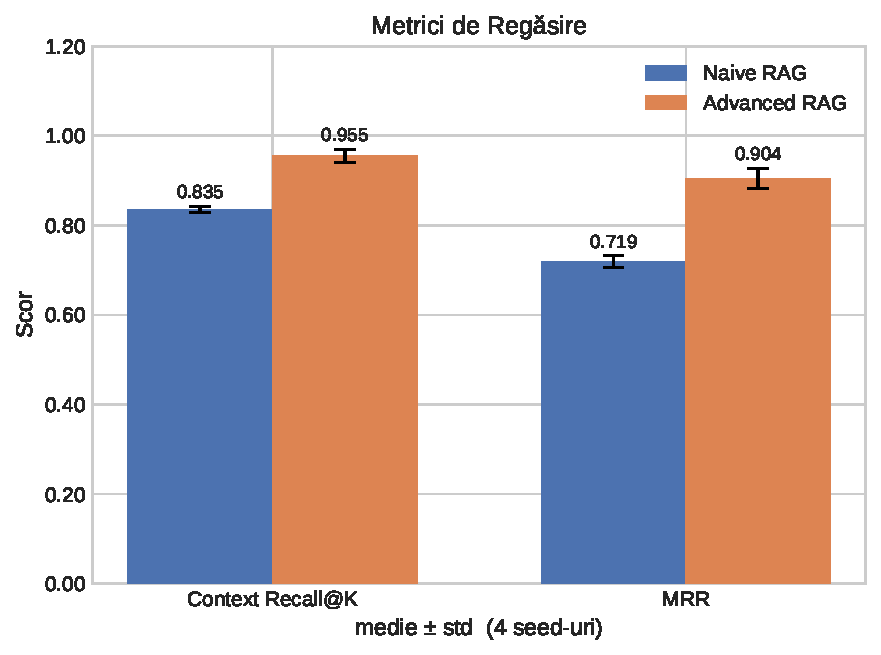
\includegraphics[width=0.80\linewidth]{Imagini/retrieval_metrics.pdf}
    \caption{Metrici de recuperare: Context Recall@5 și MRR pentru Naive RAG și Advanced RAG. Barele de eroare reprezintă deviația standard calculată pe cele 4 seed-uri.}
    \label{fig:retrieval_metrics}
\end{figure}

\begin{figure}[ht]
    \centering
    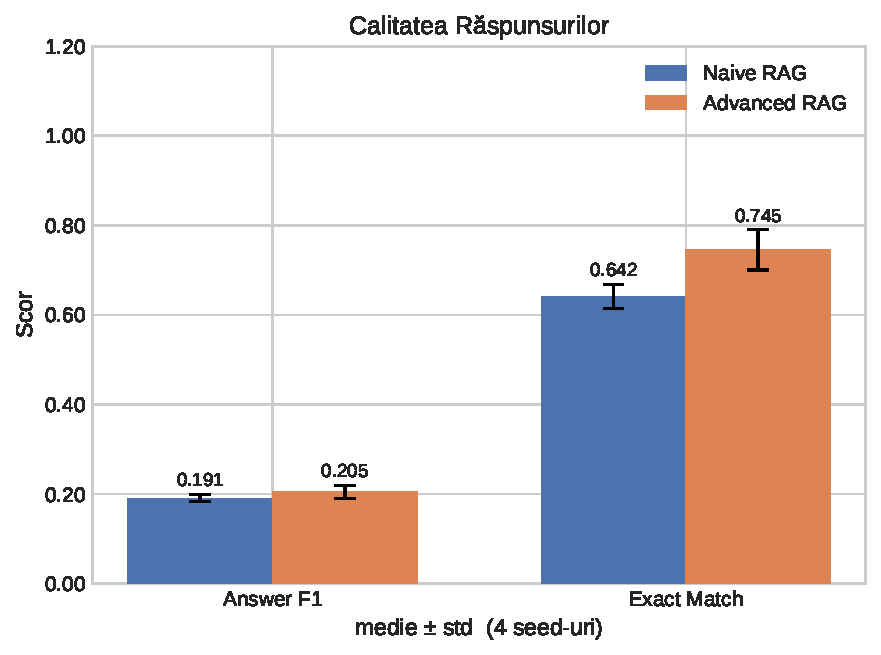
\includegraphics[width=0.80\linewidth]{Imagini/answer_quality.pdf}
    \caption{Calitatea răspunsurilor: Answer F1 și Exact Match pentru Naive RAG și Advanced RAG.}
    \label{fig:answer_quality}
\end{figure}

\begin{figure}[ht]
    \centering
    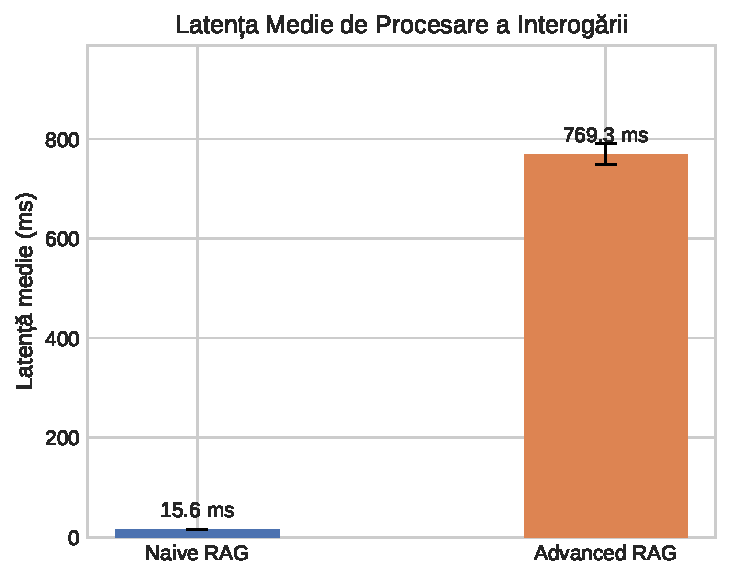
\includegraphics[width=0.65\linewidth]{Imagini/latency.pdf}
    \caption{Latența medie de procesare a interogării în milisecunde. Latența Advanced RAG include apelul LLM pentru expansiunea interogării, recuperarea hibridă paralelă și re-scorarea cu cross-encoder.}
    \label{fig:latency}
\end{figure}

\begin{figure}[ht]
    \centering
    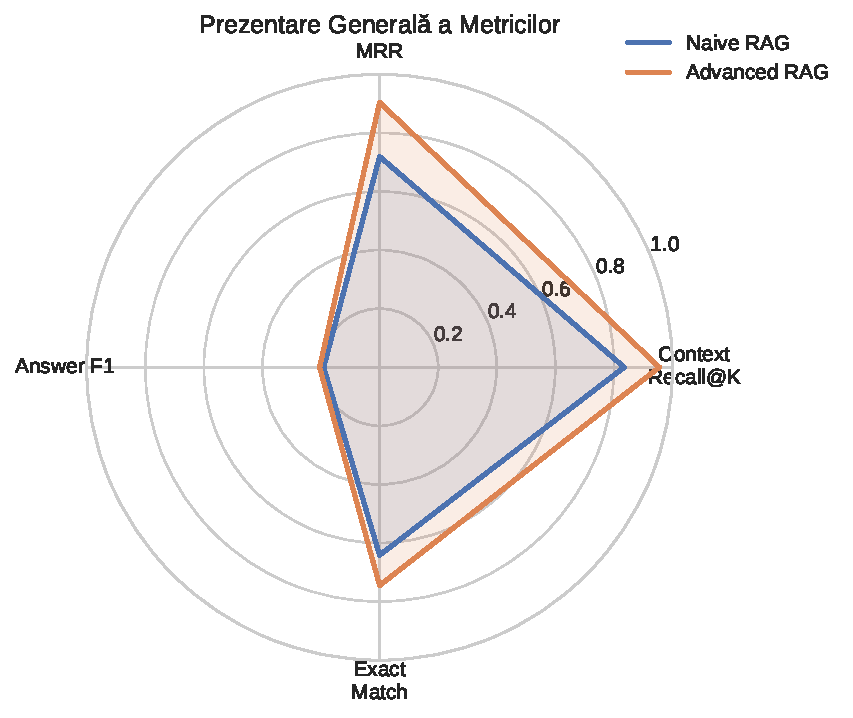
\includegraphics[width=0.72\linewidth]{Imagini/overview_radar.pdf}
    \caption{Vedere de ansamblu comparativă a metricilor de calitate (Context Recall@5, MRR, Answer F1, Exact Match). Latența nu este inclusă deoarece se află pe o scară diferită (milisecunde față de 0--1).}
    \label{fig:radar}
\end{figure}

\subsection{Semnificație statistică}

Toate diferențele observate sunt semnificative statistic la $p < 0{,}05$, cu marje considerabile față de prag (Tabelul~\ref{tab:significance}).

\begin{table}[ht]
\centering
\caption{Teste de semnificație statistică (Advanced RAG vs.\ Naive RAG, $N=600$ perechi)}
\label{tab:significance}
\begin{tabular}{lccl}
\toprule
\textbf{Metrică} & \textbf{Test} & \textbf{Valoarea $p$} & \textbf{Observații} \\
\midrule
MRR            & Wilcoxon & $6{,}5 \times 10^{-27}$ & --- \\
Answer F1      & Wilcoxon & $1{,}8 \times 10^{-3}$  & --- \\
Context Recall & McNemar  & $7{,}7 \times 10^{-20}$ & Adv.\ mai bun: 74; Naive mai bun: 2 \\
Exact Match    & McNemar  & $4{,}3 \times 10^{-10}$ & Adv.\ mai bun: 82; Naive mai bun: 20 \\
\bottomrule
\end{tabular}
\end{table}

Valoarea $p$ extrem de mică pentru MRR ($6{,}5 \times 10^{-27}$) indică o diferență sistematică, nu un artefact al eșantionării. Testul McNemar pentru Context Recall arată că există 74 de întrebări unde Advanced RAG recuperează fragmentul corect, iar Naive RAG nu reușește, față de doar 2 în situația inversă. Raportul de 37:1 în favoarea sistemului avansat confirmă că îmbunătățirile în recuperare nu provin din cazuri marginale, ci reprezintă un avantaj consistent.

\section{Analiză calitativă}

\subsection{Compromisul dintre calitate și latență}

Cel mai vizibil cost al arhitecturii avansate este latența de recuperare: 769 ms față de 16 ms pentru varianta de bază, o creștere de aproximativ 50 de ori. Această diferență are câteva surse distincte. Expansiunea interogărilor implică un apel LLM (Qwen3-1.7B), care durează câteva sute de milisecunde chiar și pentru un model de 1.7B parametri. Recuperarea densă și BM25 rulează în paralel pe toate cele trei formulări (originală plus două alternative), ceea ce limitează parțial impactul, dar cross-encoder-ul introduce o latentă suplimentară pentru re-scorarea celor 40 de candidați.

În contextul aplicațiilor RAG reale, o latență de recuperare de ~770 ms rămâne acceptabilă, deoarece generarea unui răspuns cu un model de 8B parametri durează oricum mai multe secunde. Totuși, în scenarii unde se doresc timpi de răspuns sub o secundă, overhead-ul expansiunii interogărilor devine o constrângere reală și ar putea fi eliminat printr-o versiune fără expansiune, care combină recuperarea hibridă fără reformulare~\cite{gao2024retrievalaugmentedgenerationlargelanguage}.

\subsection{Unde ajută recuperarea hibridă}

Diferența cea mai pronunțată dintre cele două sisteme apare la metricile de recuperare, nu la cele de generare. Creșterea cu 14,4 puncte la Context Recall înseamnă că, în 12 din 100 de cazuri unde Naive RAG eșuează, Advanced RAG găsește totuși fragmentul corect. MRR crescut de la 0,719 la 0,904 arată că, pe lângă faptul că găsește mai des fragmentul corect, îl și plasează pe poziții mai înalte.

Recuperarea hibridă (densă + BM25) are un avantaj clar pe interogările cu termeni specifici: date, numere, denumiri proprii, acronime. Modelul de embedding codifică înțeles semantic, dar poate dilua termeni rari într-un spațiu vectorial continuu unde similaritatea cosinus favorizează documente tematic apropiate, nu neapărat lexical identice. BM25~\cite{robertson2009bm25} nu are această problemă: un termen care apare exact o dată în corpus va fi regăsit cu precizie dacă apare și în interogare. Expansiunea interogărilor contribuie la recall prin acoperirea variantelor de formulare, reducând dependența de formularea exactă a întrebării~\cite{gao2024retrievalaugmentedgenerationlargelanguage}.

\subsection{Decalajul dintre recuperare și generare}

Îmbunătățirile la recuperare nu se traduc proporțional în îmbunătățiri la generare. Context Recall crește cu ~14 puncte procentuale, dar Answer F1 crește cu ~7\% relativ, iar Exact Match cu ~10 puncte procentuale.

Explicația principală este că SQuAD a fost conceput ca benchmark pentru citire extractivă, unde modelul ar trebui să extragă textual un fragment din pasaj. Modelele generative moderne tind să parafrazeze răspunsul mai degrabă decât să îl reproducă cuvânt cu cuvânt, ceea ce scade Answer F1 față de valoarea maximă posibilă, chiar dacă răspunsul este corect semantic. O a doua explicație este că Naive RAG recuperează corect fragmentul în 83,5\% din cazuri, ceea ce înseamnă că modelul generativ primea oricum contextul corect pentru cea mai mare parte a întrebărilor. Câștigul din Advanced RAG vine tocmai din cazurile dificile, adică interogările cu termeni rari sau cu răspunsuri scurte greu de localizat prin similaritate semantică pură, unde generarea oricum eșuează mai des.

\subsection{Constrângerea de groundare și refuzurile}

Ambele pipeline-uri folosesc un prompt de sistem care constrânge modelul să răspundă exclusiv din contextul furnizat și să refuze explicit dacă informația lipsește. Exact promtul de refuz este: \textit{``The provided context does not contain enough information to answer this question.''} Această decizie de proiectare este direct motivată de principiul fidelității contextuale descris în~\cite{asai2023self}: un sistem care preferă să refuze decât să inventeze este mai fiabil decât unul care generează răspunsuri plauzibile dar incorecte.

Refuzurile nu pot fi evaluate cu Answer F1 sau Exact Match, deoarece nu conțin conținut factual comparabil cu referința. Advanced RAG generează mai puține refuzuri decât Naive RAG, pentru că recuperează mai frecvent fragmentul corect și îl plasează pe primele poziții, astfel că modelul primește mai rar un context din care nu poate răspunde.

\subsection{Observații calitative din interfața Streamlit}

Interfața Streamlit permite observarea directă a diferențelor de comportament fără a parcurge metricile agregate.

Pe întrebări cu termeni numerici sau coduri specifice (``Câte specii...'', ``În ce an...'', ``Care este codul...''), Naive RAG returnează adesea fragmente tematic relevante care nu conțin numărul exact. Advanced RAG găsește fragmentul corect prin BM25, care tratează numerele ca termeni distincți și nu le diluează în spațiu vectorial.

Când răspunsul nu există în corpus, ambele sisteme refuză explicit. Diferența este că Advanced RAG produce mai rar răspunsuri parțiale construite din context adiacent irelevant, deoarece cross-encoder-ul elimină candidații slab relevanți înainte de generare.

Pe întrebări tematice generale (``Despre ce este...'', ``Care este rolul...''), ambele sisteme produc rezultate similare. Recuperarea densă funcționează bine pe similitudine semantică, iar avantajul hibridizării este mai puțin pronunțat în aceste cazuri.

Aceste observații sunt consistente cu rezultatele cantitative: câștigurile Advanced RAG sunt mai mari pe cazurile dificile (termeni rari, răspunsuri numerice) și mai mici pe interogările tematice generale, unde recuperarea densă funcționează deja bine~\cite{gao2024retrievalaugmentedgenerationlargelanguage,robertson2009bm25}.

\chapter*{Concluzii}
\addcontentsline{toc}{chapter}{Concluzii}

\section*{Rezultate obținute}

Lucrarea a urmărit două obiective paralele: un studiu al literaturii de specialitate privind sistemele de tip Retrieval-Augmented Generation (RAG) și implementarea unui demonstrator care compară o arhitectură de bază cu una avansată pe un set de date public.

Din studiul de literatură (Capitolul 1) au reieșit câteva concluzii clare. Problema fundamentală pe care o adresează RAG rămâne aceeași ca la apariția termenului în 2020~\cite{lewis2020rag}: modelele lingvistice mari au cunoștințe fixate la momentul antrenării și generează răspunsuri incorecte atunci când nu dețin informația solicitată. RAG rezolvă această limitare nu prin reantrenare, ci prin recuperarea documentelor relevante la momentul interogării și condiționarea generării pe aceste documente. Diversitatea abordărilor din literatură, de la Naive RAG la arhitecturi modulare și grafuri de cunoștințe~\cite{gao2024retrievalaugmentedgenerationlargelanguage,peng2025graph}, reflectă că nu există o soluție universală: alegerea arhitecturii depinde de tipul sursei de date, de latența acceptabilă și de natura sarcinii.

Studiul a identificat că metodele de recuperare hibridă (densă + BM25~\cite{robertson2009bm25}) și reranking-ul cu cross-encoder aduc cele mai consistente îmbunătățiri față de recuperarea densă pură, în special pe interogări cu termeni rari sau numerici. Metodele adaptive precum Self-RAG~\cite{asai2023self} și CRAG~\cite{yan2024crag} adaugă un nivel de auto-evaluare a calității recuperării, reducând halucinațiile cauzate de documente irelevante. Pentru extragerea relațiilor între entități, abordările bazate pe grafuri de cunoștințe~\cite{edge2024graphrag} sunt cele mai potrivite structural, deoarece relațiile sunt reprezentate explicit și pot fi traversate direct.

Analiza metodelor a arătat și o tendință de evoluție a domeniului: de la pipeline-uri liniare fixe, spre sisteme care evaluează și corectează adaptiv calitatea recuperării, și mai departe spre arhitecturi care structurează explicit cunoștințele sub formă de graf. Fiecare pas pe acest drum aduce un câștig de capacitate, dar și un cost suplimentar de complexitate și de calcul. Niciuna dintre metode nu domină pe toate criteriile; alegerea potrivită depinde de tipul datelor, de latența acceptabilă și de natura sarcinii. Această observație justifică abordarea adoptată în lucrare, de a porni de la o arhitectură simplă și de a măsura efectul fiecărei optimizări, în loc de a implementa direct cea mai complexă variantă.

Din evaluarea experimentală (Capitolul 2) rezultatele arată că Advanced RAG depășește Naive RAG pe toate metricile de calitate, cu diferențe semnificative statistic ($p \ll 0{,}05$ în toate testele). Context Recall@5 a crescut de la 83,5\% la 95,5\% (+12,0 puncte procentuale), MRR de la 0,719 la 0,904 (+0,185), iar Exact Match de la 64,2\% la 74,5\% (+10,3 puncte procentuale). Testul McNemar pentru Context Recall a arătat că există 74 de întrebări unde Advanced RAG recuperează fragmentul corect iar Naive RAG nu, față de doar 2 în situația inversă, un raport de 37:1 în favoarea arhitecturii avansate.

Costul acestor îmbunătățiri este latența: Advanced RAG necesită ~770 ms per interogare față de ~16 ms pentru Naive RAG, o diferență de aproximativ 50 de ori. Cea mai mare parte a acestui overhead provine din apelul LLM pentru expansiunea interogărilor. În aplicații unde latența de recuperare poate fi ascunsă parțial de latența de generare (care durează oricum câteva secunde pentru modele de 8B parametri), compromisul este acceptabil. Îmbunătățirile la Answer F1 au fost mai modeste (7,3\% relativ), ceea ce este de așteptat: SQuAD este un benchmark extractiv, iar modelele generative modifică formularea răspunsului chiar și atunci când contextul corect este disponibil.

Analiza pe seed-uri și testele de semnificație confirmă că aceste rezultate sunt stabile și reproductibile, nu artefacte ale unui eșantion particular. Advanced RAG depășește varianta de bază pe fiecare seed în parte, iar analiza erorilor arată că cele câteva cazuri în care Naive RAG răspunde mai bine se explică prin reformulări nereușite ale interogării sau prin limitele metricii Exact Match, nu printr-un avantaj real al recuperării simple. Per ansamblu, studiul de literatură și partea experimentală conduc la aceeași concluzie: în sistemele RAG, calitatea recuperării este pârghia principală asupra calității răspunsului.

\section*{Contribuții originale}

Contribuția principală a lucrării este demonstratorul implementat, disponibil ca proiect open-source, care compară Naive RAG și Advanced RAG pe același set de date și același model lingvistic, izolând contribuția etapelor de recuperare. Sistemul rulează local prin Ollama și ChromaDB, fără dependență de servicii externe.

Din punct de vedere tehnic, Advanced RAG adaugă patru optimizări față de varianta de bază. Recuperarea hibridă combină recuperarea densă (all-MiniLM-L6-v2~\cite{karpukhin2020dpr} + ChromaDB) cu recuperarea sparse (BM25~\cite{robertson2009bm25} prin \texttt{bm25s}), listele rezultate fuzionând prin Reciprocal Rank Fusion~\cite{cormack2009rrf}. Expansiunea interogărilor folosește Qwen3-1.7B pentru a genera două reformulări ale interogării originale, reducând dependența de formularea exactă. Reranking-ul cu cross-encoder (\texttt{ms-marco-MiniLM-L-6-v2}) re-scorează cele mai bune 40 de candidate și returnează primele 5. Ambele sisteme refuză explicit când contextul recuperat nu conține informația solicitată, în loc să genereze răspunsuri plauzibile dar incorecte~\cite{asai2023self}.

Scriptul de benchmark suportă evaluare pe mai multe seed-uri cu checkpoint după fiecare run, teste de semnificație statistică (Wilcoxon și McNemar) și generare automată de figuri. Interfața Streamlit permite testarea interactivă a ambelor sisteme și vizualizarea comparativă a răspunsurilor.

Taxonomia din Capitolul 1 a fost adaptată pentru extragerea relațiilor între entități, nu pentru domeniul RAG în ansamblu, ceea ce limitează acoperirea dar face clasificarea mai directă pentru înțelegerea alegerii arhitecturale din demonstrator.

Dincolo de cifrele de performanță, demonstratorul are valoare ca instrument de comparație: pentru că ambele sisteme rulează pe aceeași bază și pot fi interogate simultan, diferențele de comportament devin vizibile direct, nu doar prin metrici agregate. Interfața permite observarea felului în care recuperarea hibridă recuperează termeni pe care recuperarea densă îi ratează, sau a felului în care constrângerea de groundare conduce la un refuz explicit în locul unei halucinații. Această transparență face din demonstrator un punct de plecare util atât pentru extinderea către extragerea relațiilor, cât și pentru înțelegerea practică a compromisurilor descrise teoretic în studiul de literatură.

\section*{Perspective de dezvoltare ulterioară}

O limitare concretă a evaluării actuale este că s-a realizat pe SQuAD, un set de date de tip QA extractiv. Lucrarea urmărește aplicarea RAG la extragerea relațiilor între entități, pentru care T-REx~\cite{elsahar2018trex} (aliniament Wikipedia-Wikidata) sau DocRED~\cite{yao2019docred} sunt mai potrivite structural, deoarece conțin triplete (subiect, predicat, obiect) explicit adnotate. Adaptarea benchmark-ului pentru aceste seturi rămâne pasul imediat următor.

Evaluarea RAGAS~\cite{es2024ragas}, cu metrici de fidelitate (faithfulness) și relevanță a răspunsului (answer relevancy), nu a putut fi finalizată în limitele de timp disponibile din cauza costului computațional ridicat (modelul judecător rulează câte un apel LLM per pereche întrebare-răspuns). O evaluare completă ar adăuga perspectiva calității fundamentării în context, independentă de potrivirea textuală cu referința.

Pe latura arhitecturală, GraphRAG~\cite{edge2024graphrag} și HippoRAG~\cite{gutierrez2024hipporag} indexează explicit relațiile dintre entități și le utilizează la recuperare, ceea ce le face candidați direcți pentru extragerea relațiilor față de pipeline-urile actuale bazate pe fragmente de text. O comparație extinsă cu aceste metode ar clarifica în ce măsură structura relațională explicită aduce beneficii față de recuperarea hibridă pe text nestructurat.

Latența Advanced RAG (~770 ms per interogare) provine în cea mai mare parte din apelul LLM pentru expansiunea interogărilor. O variantă fără expansiune, care păstrează recuperarea hibridă și cross-encoder-ul, ar reduce latența la câteva zeci de milisecunde cu o pierdere relativ mică la recall. Această variantă ar fi utilă în scenarii cu constrângeri stricte de timp de răspuns.

Evaluarea actuală folosește Qwen3-8B ca model generativ, fără fine-tuning. Modele mai mari sau antrenate specific pe extragerea relațiilor pot produce îmbunătățiri la Answer F1 independent de arhitectura de recuperare. Separarea contribuției modelului generativ de contribuția pipeline-ului de recuperare rămâne o direcție deschisă pentru cercetare ulterioară.

O direcție complementară privește extinderea evaluării dincolo de limba engleză. SQuAD și majoritatea seturilor de date folosite sunt în engleză, iar comportamentul sistemului pe texte în alte limbi, inclusiv în română, rămâne neexplorat. Modelul de embedding și cel generativ folosite au capacități multilingve, dar calitatea recuperării și a extragerii relațiilor pe corpusuri în limba română ar trebui măsurată separat, deoarece resursele și performanța modelelor diferă semnificativ între limbi. O astfel de evaluare ar fi relevantă pentru aplicarea sistemului pe documente locale, unde nevoia de extragere a relațiilor este la fel de prezentă.

Per ansamblu, lucrarea confirmă pe un caz concret o observație recurentă din literatură: în sistemele RAG, calitatea recuperării este factorul determinant pentru calitatea răspunsului final. Optimizările aduse de Advanced RAG, deși nu sunt complexe, produc îmbunătățiri consistente și semnificative statistic, la un cost de latență acceptabil pentru cele mai multe aplicații. Această concluzie justifică direcția aleasă și oferă o bază solidă pentru pasul următor, aplicarea și evaluarea aceleiași arhitecturi pe extragerea relațiilor între entități, scopul final al cercetării.


% ======================================================
% BIBLIOGRAFIE
% ======================================================
\bibliographystyle{unsrt}
\bibliography{referinte}

% ======================================================
% ANEXE (numerotate incepand cu Anexa 1)
% ======================================================
\appendix
%\include{Anexe/anexa_1}
%\include{Anexe/anexa_n}

\end{document}
